 \documentclass{beamer}
\beamertemplatenavigationsymbolsempty
\usepackage{amsmath, amssymb, hyperref, graphics, tikz}
%\usepackage{mathpazo, soul}



\newcommand{\C}{\mathbb{C}}
\newcommand{\Z}{\mathbb{Z}}
\newcommand{\R}{\mathbb{R}}
\newcommand{\N}{\mathbb{N}}
\DeclareMathOperator{\Real}{Re}
\DeclareMathOperator{\Imag}{Im}


\begin{document}



\begin{frame}{``ML-bounds'': M=Maximum, L=Length}
\begin{theorem} Suppose that $f$ is continuous on a path $\gamma$ of length $L$, and that $|f(z)|\leq M$ on $\gamma$.  Then $|\int_\gamma f dz|\leq ML$
\end{theorem}
\begin{proof}\begin{align*}
    \left|\int_\gamma f(z)dz\right|&=\left|\int_a^b f(z(t))z^\prime(t)dt\right| \\
    &\leq \int_a^b |f(z(t))| |z^\prime(t)| dt \\
    &\leq \int_a^b M |z^\prime(t)| dt = ML
\end{align*}
\end{proof}
The second line is triangle inequality for integrals.
\end{frame}
\begin{frame}{Applications of the ML-inequality}
\begin{block}{Why do ML-inequalities?}
The ML-inequality will help prove two of our big theorems.  \\
We will take limits of paths where $M$ or $L$ are going to zero, and conclude the integral goes to zero.
\end{block}
\alert{``Toy'' uses appear on exam}
\begin{example}[From notes]
Let $\gamma$ be a line segment lying with $D=\{z\in\C: |z|<1$.  Give an upper bound for 
$$\int_\gamma \left(\frac{\Real{z}+z^2}{3+\overline{z}}\right)dz$$
\end{example}

\end{frame}

\begin{frame}{Section 8: Cauchy's Theorem}

\begin{theorem}[Cauchy's Theorem] Suppose the function $f$ is analytic on a \alert{simply connected} region $D$.  Then $\int_\gamma fdz=0$ for \emph{all} contours $\gamma$ in $D$.
\end{theorem}
\begin{example}
$$\int_{C_{0,1/2}} \frac{\sin(e^{3z}\cos(z))}{1+z^3}dz=0$$
\end{example}

\begin{example}[Necessary to ask that $D$ is simply connected]
The function $1/z$ is analytic on $\C\setminus\{0\}$.  Letting $\gamma=e^{it}, 0\leq t\leq 2\pi$ we have 
$$\int_\gamma \frac{1}{z} dz=2\pi i$$
No Cauchy, because $\C\setminus\{0\}$ isn't simply connected.
\end{example}
\end{frame}
\begin{frame}{I didn't agree with these quotes in the notes}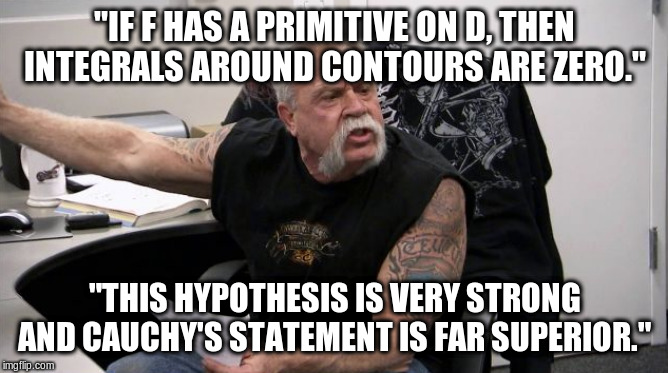
\includegraphics[width=\textwidth,height=0.8\textheight,keepaspectratio]{ChopperFilled1.jpg}
\end{frame}
\begin{frame}{Here's why:}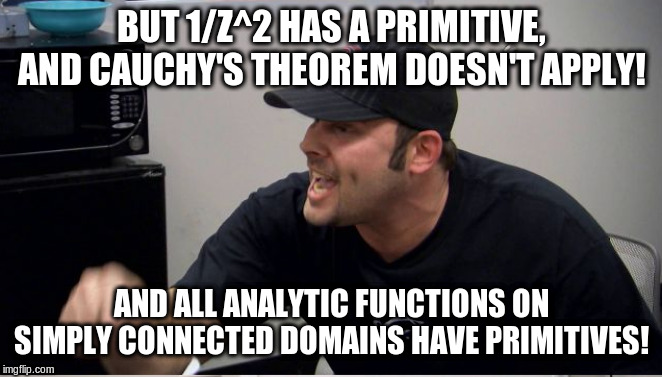
\includegraphics[width=\textwidth,height=0.8\textheight,keepaspectratio]{ChopperFilled2.jpg}
\begin{itemize}
    \item Can prove $\int_{C_1(0)}\frac{1}{z^2}dz=0$ using primitives, not Cauchy
    \item Hypotheses of Cauchy will tell us $f$ \emph{has} a primitive
\end{itemize}
\end{frame}
\begin{frame}{Mary's rebuttal}
\includegraphics[width=\textwidth,height=0.8\textheight,keepaspectratio]{ChopperFilled3.jpg}
To prove that $f$ analytic, $D$ simply connected $\implies$ $f$ has primitive comes much later in notes, and \emph{depends} on Cauchy's theorem.
\end{frame}
\begin{frame}{Well, sure, but...}
\includegraphics[width=\textwidth,height=0.8\textheight,keepaspectratio]{ChopperFilled4.jpg}
The pay-off for Cauchy's theorem doesn't come until later
\end{frame}
\begin{frame}{We're in agreement after all...}
\includegraphics[width=\textwidth,height=0.8\textheight,keepaspectratio]{ChopperFilled5.jpg}
Even if I disagree about Cauchy being superior, I agree the point is that the hypotheses of Cauchy's Theorem are very weak
\end{frame}
\begin{frame}{The proof of Cauchy's Theorem}
\begin{block}{The proof of Cauchy's Theorem is hard}
Because the hypotheses are so weak!
\begin{itemize}
    \item We won't prove it
    \item Notes: Green's Theorem + Cauchy-Riemann would prove it
    \item But Green's theorem requires \emph{continuous} partial derivatives; we only have that $f$ has a derivative!
\end{itemize}
Proof \emph{is} in the recommended textbooks...
\end{block}
\begin{example}[A non-continuous derivative]
$$f(x)=\begin{cases}x^2\sin(1/x) & x\neq 0\\0 & x=0 \end{cases}$$
$$f^\prime(x)=\begin{cases}2x\sin(1/x)-\cos(1/x) & x\neq 0\\0 & x=0 \end{cases}$$
\end{example}

\end{frame}

\end{document}
